\documentclass[12pt,a4paper]{article}
\usepackage{graphicx}
\usepackage{geometry}
\usepackage{xcolor}
\usepackage{array}
\usepackage{longtable}
\usepackage{fancyhdr}
\usepackage{amsmath}
\geometry{margin=1in}

\setlength{\headheight}{65pt}

\begin{document}

\begin{center}
    \Large\textbf{\color{blue}Gate CS 2010,Qustion no.6}
\end{center}

\thispagestyle{fancy}
\fancyhf{}
\fancyhead[L]{\includegraphics[height=1.5cm]{LOGO.PNG}}
\fancyhead[R]{
\begin{tabular}{r}
\textbf{Name: Pavan Kumar KS} \\
\textbf{ID: COMETFWC044} \\
\textbf{Date: 19 Jan 2026}
\end{tabular}
}
\renewcommand{\headrulewidth}{0.4pt}

\vspace{0.5cm}

%---------------- QUESTION ----------------%

\section*{\color{blue}QUESTION}}

The minterm expansion of
\[
F = PQ + QR' + PR'
\]


\begin{tabular}{ll}
(A) $m_2 + m_4 + m_6 + m_7$ 
& (B) $m_0 + m_1 + m_4 + m_5$ \\[0.4cm]

(C) $m_0 + m_1 + m_6 + m_7$ 
& (D) $m_2 + m_3 + m_6 + m_7$ \\
\end{tabular}


%---------------- QUESTION ANALYSIS ----------------%

\section*{\color{blue}QUESTION ANALYSIS}}


\[
F = PQ + QR' + PR'
\]

Where:
\begin{itemize}
\item P, Q, R are input variables
\item R' is complement of R
\item '+' represents OR operation
\item Concatenation represents AND operation
\end{itemize}

Output will be displayed as:
\begin{itemize}
\item 0 when expression evaluates to 0
\item 1 when expression evaluates to 1
\end{itemize}

%---------------- TRUTH TABLE ----------------%

\section*{\color{blue}TRUTH TABLE}}

\begin{center}
\begin{tabular}{|c|c|c|c|}
\hline
P & Q & R & F \\
\hline
0 & 0 & 0 & 0 \\
0 & 0 & 1 & 0 \\
0 & 1 & 0 & 1 \\
0 & 1 & 1 & 0 \\
1 & 0 & 0 & 1 \\
1 & 0 & 1 & 0 \\
1 & 1 & 0 & 1 \\
1 & 1 & 1 & 1 \\
\hline
\end{tabular}
\end{center}

Minterm form:
\[
F = \Sigma m(2,4,6,7)
\]

%---------------- HARDWARE IMPLEMENTATION ----------------%

\section*{\color{blue}HARDWARE IMPLEMENTATION}}

The Boolean expression is implemented using:
\begin{itemize}
\item Arduino UNO (ATmega328P)
\item 7447 BCD to 7-segment decoder
\item Common Anode 7-segment display
\end{itemize}

Inputs are given through PORTD pins and output is sent through PORTB to 7447.

%---------------- COMPONENTS REQUIRED ----------------%

\section*{\color{blue}COMPONENTS REQUIRED}}

\begin{center}
\begin{tabular}{|c|l|}
\hline
Sl.No & Component \\
\hline
1 & Arduino UNO \\
2 & 7447 IC \\
3 & Common Anode 7-Segment Display \\
4 & 220$\Omega$ Resistors (7 Nos) \\
5 & Breadboard \\
6 & Connecting Wires \\
\hline
\end{tabular}
\end{center}

%---------------- PIN CONNECTIONS ----------------%

\section*{\color{blue}PIN CONNECTIONS}}

\textbf{Input Connections}

\begin{center}
\begin{tabular}{|c|c|c|}
\hline
Variable & Arduino Pin & AVR Port \\
\hline
P & D2 & PD2 \\
Q & D3 & PD3 \\
R & D4 & PD4 \\
\hline
\end{tabular}
\end{center}

\textbf{Output Connections (To 7447)}

\begin{center}
\begin{tabular}{|c|c|c|}
\hline
7447 Pin & Arduino Pin & AVR Port \\
\hline
A & D8 & PB0 \\
B & D9 & PB1 \\
C & D10 & PB2 \\
D & D11 & PB3 \\
\hline
\end{tabular}
\end{center}

%---------------- LOGIC DESCRIPTION ----------------%

\section*{\color{blue}LOGIC DESCRIPTION}}

The program reads inputs P, Q and R from PORTD.

\begin{itemize}
\item R is complemented to generate R'
\item AND operations compute PQ, QR', and PR'
\item OR operation combines all terms
\item Result is sent as BCD to 7447
\end{itemize}

If F = 0, display shows 0.  
If F = 1, display shows 1.

%---------------- CODE UPLOADING STEPS ----------------%

\section*{\color{blue}CODE UPLOADING STEPS}}

\begin{enumerate}
\item Create a folder
\item Write the code in filename.asm
\item Run the command ``avra filename.asm''. It will compile the code and creates hex file
\item Copy the .hex file to ArduinoDriod folder
\item Connect the Arduino UNO to mobile with OTG cable
\item Upload the hex file using ``upload precompiled'' option
\item Observe the output and verify the expression
\end{enumerate}

%---------------- EXPERIMENTAL TRUTH TABLE ----------------%

\section*{\color{blue}EXPERIMENTAL TRUTH TABLE}}

\begin{center}
\begin{tabular}{|c|c|c|c|}
\hline
P & Q & R & Observed F \\
\hline
0 & 0 & 0 & 0 \\
0 & 0 & 1 & 0 \\
0 & 1 & 0 & 1 \\
0 & 1 & 1 & 0 \\
1 & 0 & 0 & 1 \\
1 & 0 & 1 & 0 \\
1 & 1 & 0 & 1 \\
1 & 1 & 1 & 1 \\
\hline
\end{tabular}
\end{center}

%---------------- CIRCUIT CONNECTION ----------------%

\section*{\color{blue}CIRCUIT CONNECTION}}

\begin{center}
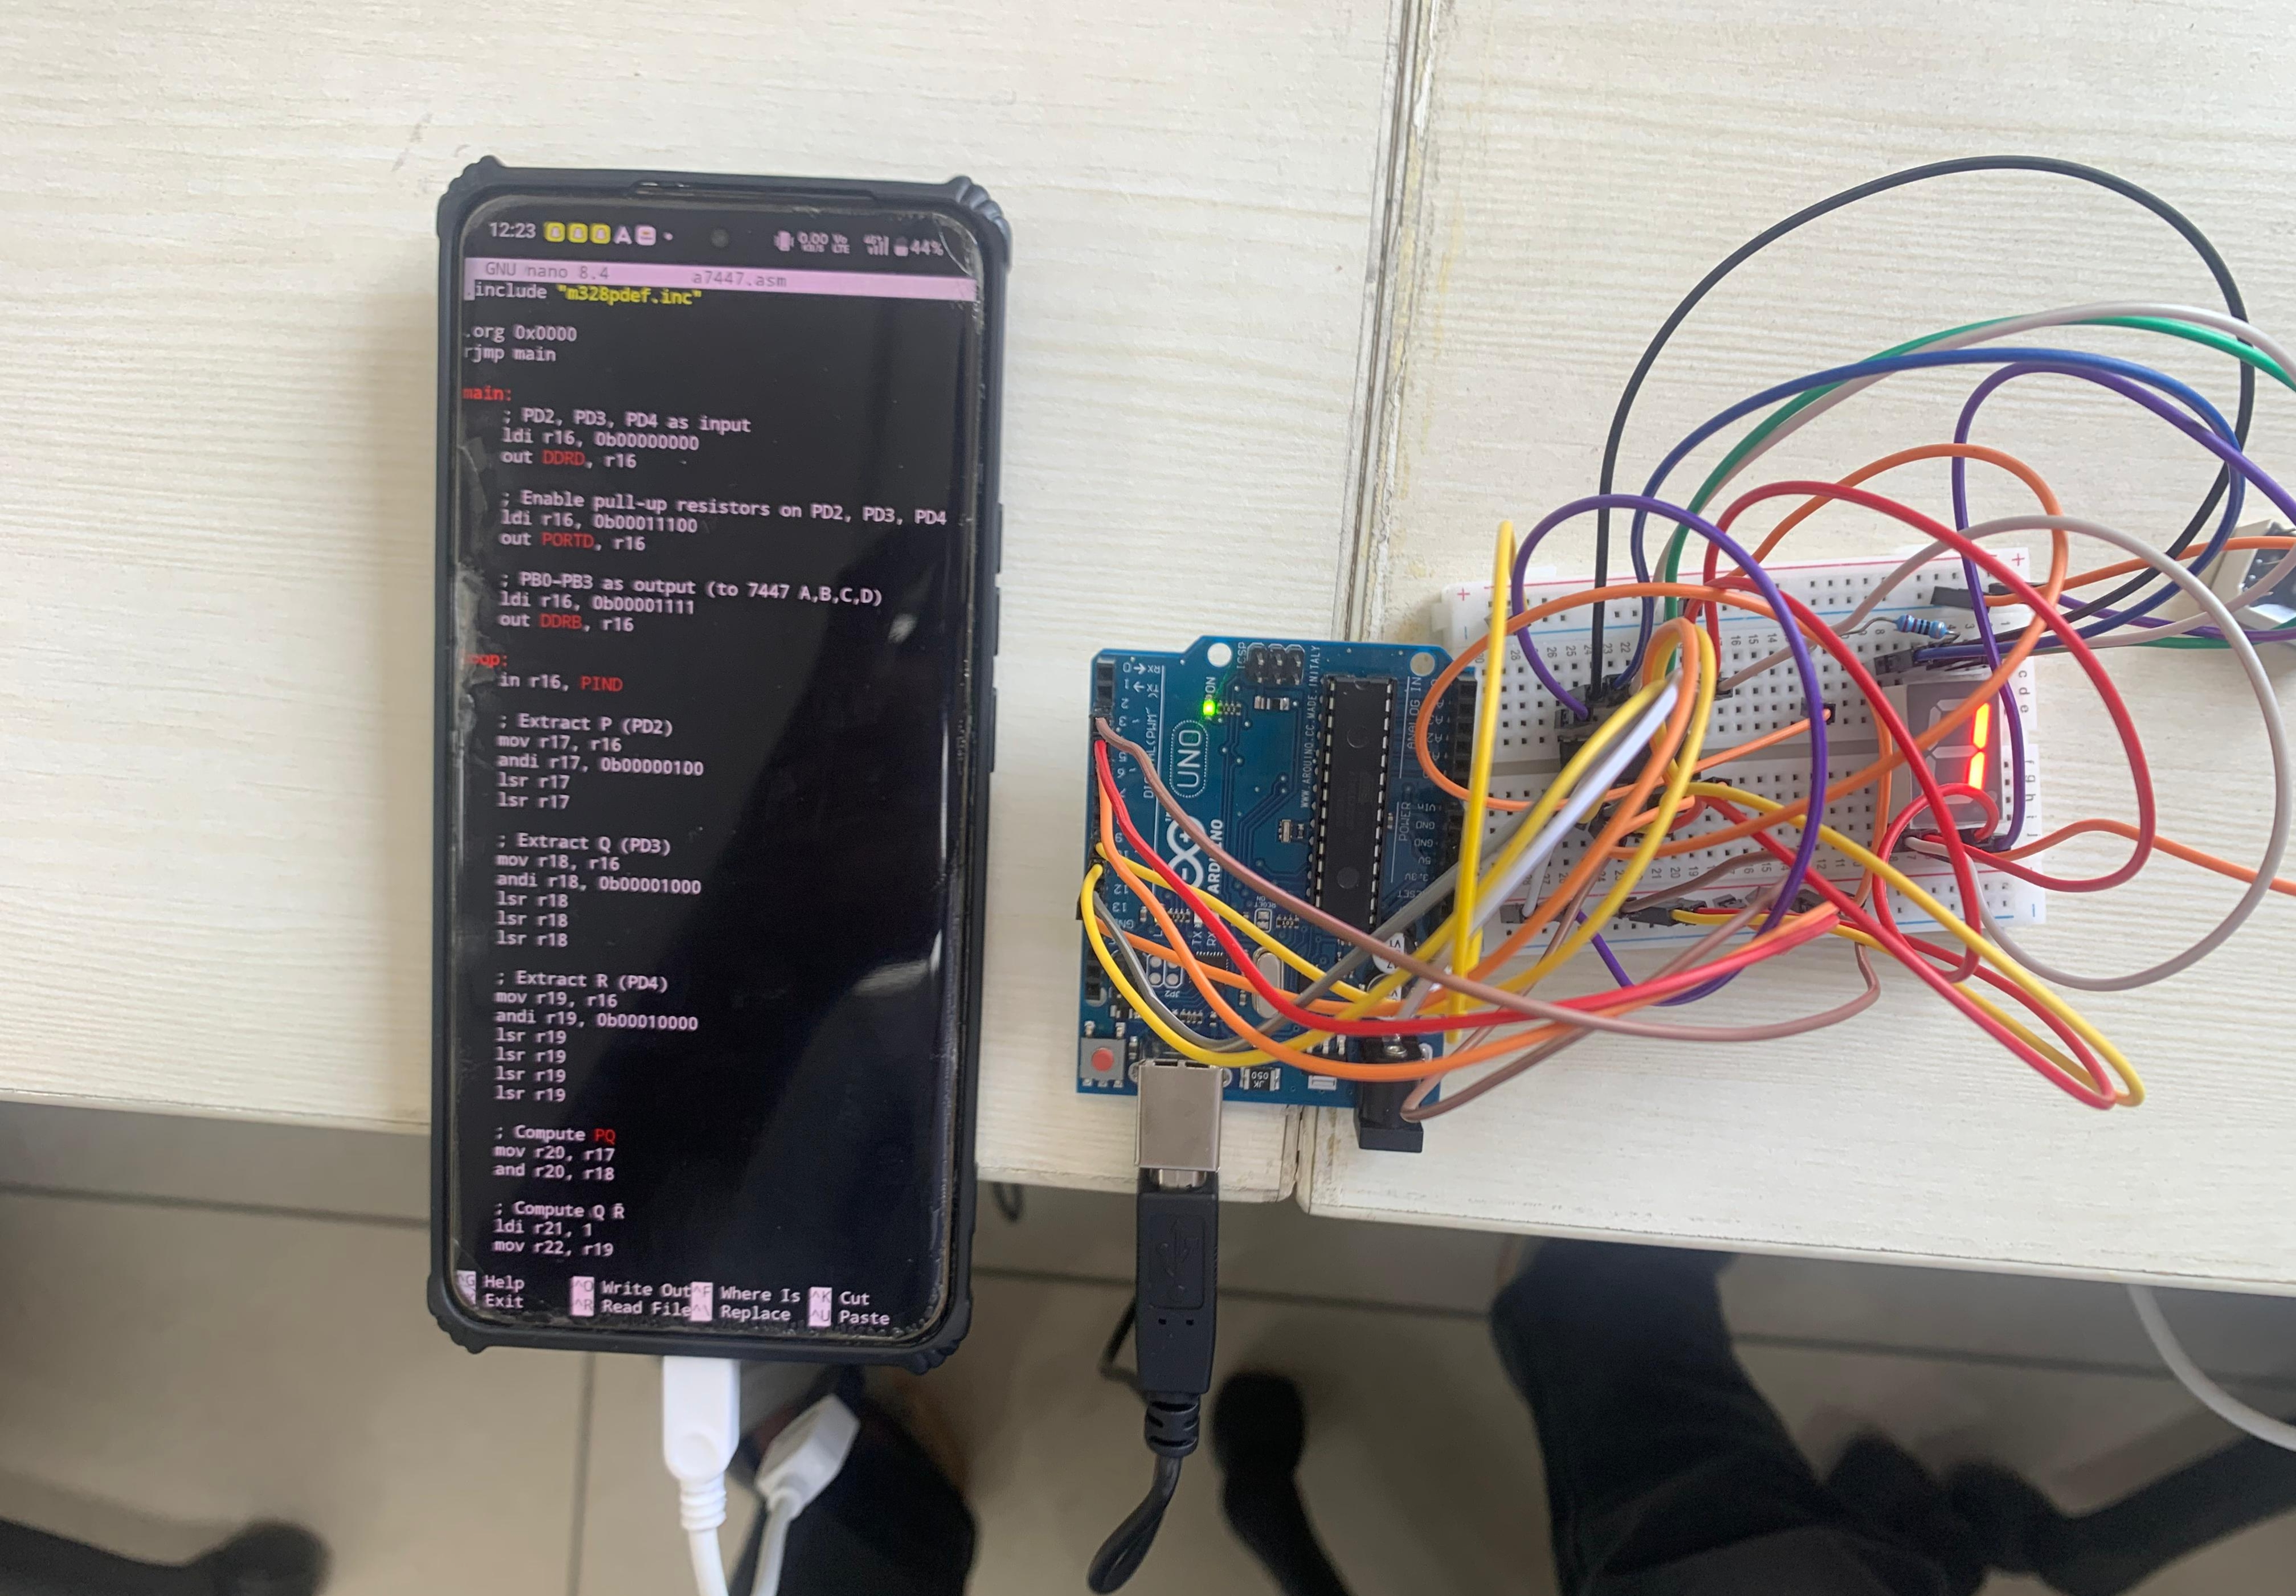
\includegraphics[width=0.8\textwidth]{pic.jpg}
\end{center}

%---------------- CONCLUSION ----------------%

\section*{\color{blue}CONCLUSION}}

The Boolean expression \(F = PQ + QR' + PR'\) was successfully implemented using AVR Assembly language.  
The output was verified using 7447 decoder and Common Anode 7-segment display.

\end{document}
